\documentclass{article}
\usepackage{graphicx,fancyhdr,amsmath,amssymb,amsthm,subfig,url,hyperref}
\usepackage[margin=1in]{geometry}
\usepackage{booktabs}
\usepackage{enumitem}
\usepackage{bbm}
\usepackage{multicol,tabularx,capt-of}
\usepackage{multirow}
\usepackage{hhline}% http://ctan.org/pkg/hhline
\usepackage{array}
\usepackage{float}
%\usepackage{minted}
\usepackage{bm}
\usepackage{bbm}
\usepackage{subfloat}


%----------------------- Macros and Definitions --------------------------

%%% FILL THIS OUT
\newcommand{\studentname}{Nolan Skochdopole, Lan Huong Nguyen}
\newcommand{\suid}{naskoch, lanhuong}
\newcommand{\exerciseset}{}
%%% END

\theoremstyle{plain}
\newtheorem{theorem}{Theorem}
\newtheorem{lemma}[theorem]{Lemma}

\theoremstyle{definition}
\newtheorem{definition}{Definition}[section]

\fancypagestyle{plain}{}
\pagestyle{fancy}
\fancyhf{}
\fancyhead[RO,LE]{\sffamily\bfseries\large Stanford University}
\fancyhead[LO,RE]{\sffamily\bfseries\large CS 269I Incentives in Computer Science}
\fancyfoot[LO,RE]{\sffamily\bfseries\large \studentname: \suid @stanford.edu}
\fancyfoot[RO,LE]{\sffamily\bfseries\thepage}
\renewcommand{\headrulewidth}{1pt}
\renewcommand{\footrulewidth}{1pt}

\graphicspath{{figures/}}

%-------------------------------- Title ----------------------------------

\title{Loyalty Based Bitcoin Mining Reward Functions}
\author{\studentname \qquad SUNet ID: \suid}

%--------------------------------- Text ----------------------------------

\begin{document}
\maketitle

\begin{abstract}
Bitcoin miners join mining pools in an effort to decrease their payoff variances. These pools distribute rewards to their miners for each new block found according to some pre-specified reward functions. Ideally, everyone's expected revenue in pools would be equal to that of solo-mining (minus some small fees to pool operators). However, miners may sometimes strategically hop between pools to earn more than their share of revenue. Some pool reward functions have already been designed to combat this behavior\cite{Rosefeld2011}. In this paper, we develop a new class of reward functions based on miner loyalty to also address pool-hopping. These new reward functions specifically punish miners for hopping behavior, whereas previous methods do not explicitly do this. We define this class of functions and analyze a simple example, the badge system. Through simulations, we characterize when people will hop from this type of pool. We show that these types of reward functions discourage hopping to a similar level that existing methods do. Finally, this new loyalty concept may be easily combined with existing reward functions\footnote{Video presentation can be found here: \url{https://youtu.be/-9gMbsKohmw}}
\end{abstract}

\section{Introduction}
Cryptocurrencies have become a very popular decentralized medium of exchange over the last decade, commanding billions of US dollars in market value. Bitcoin is by far the most popular of these cryptocurrencies and represents the majority of their market cap \footnote{\url{https://coinmarketcap.com/}}. The Bitcoin system relies on a globally accepted public ledger, known as the \emph{blockchain}. Transactions are added to the blockchain through the process of \emph{mining}: solving difficult cryptopuzzles to find a valid block containing pending transactions to add to the blockchain. People spend computing resources to solve these cryptopuzzles because they are rewarded with newly created Bitcoins (a flat reward, not dependent at all on the contents of the block) as well as some transaction fees (dependent on the contents of the block) when they mine a new valid block\footnote{See class notes (\url{http://theory.stanford.edu/~tim/f16/l/l9.pdf} for more details on Bitcoin system.}.

New blocks are very valuable, but they are also very difficult to find. Individual miners face a very large revenue variance; solo miners only make revenue when they find a valid block, which happens very infrequently. This incredible revenue volatility encourages miners to form \emph{pools}, in which miners effectively boost their computational power and share profits in some agreed upon fashion, lowering revenue variance. Pools are managed by operators who charge fees usually proportional to the total profit generated by the miners. Thus, miners entering pools trade some of their expected revenue to decrease their revenue variance. Pool operators must distribute rewards for each block found according to some \emph{reward function}.

In this paper, we develop a new class of pool reward functions, which we call \emph{loyalty reward functions}. Most previous reward functions implemented and studied have focused on proportional payments\cite{Rosefeld2011}\cite{tim}. However, many of these reward systems have been shown to be susceptible to an attack called ``pool-hopping''\cite{Rosefeld2011}, in which a miner may strategically hop between mining pools to increase his own revenue. Although some research already exists into reward functions that combat pool-hopping, we argue that these systems are not strong enough. Therefore, we introduce loyalty reward functions as a new method to combat pool-hopping. Pools adopting these reward system explicitly punish hopping from their pools, whereas no other existing reward functions do this.

\section{Previous Work}
First we go through some preliminary definitions and notation. The computational power of miner $i$ is denoted by $\alpha_i$. Because the best algorithm for solving the Bitcoin cryptopuzzles is simple brute-force, the probability of each miner finding a new block will be directly proportional to his computational power. We assume this value is normalized, so $\sum_{i} \alpha_i = 1$. We will call $p({\alpha})$ the computational power of a pool $p$: $p_\alpha = \sum_{i\in p} \alpha_i$.

The time period between finding new blocks within a pool is known as a \emph{round}. Each time the pool finds a new block, it distributes the reward to the miners who were involved with the pool during that round, according to its adopted reward function. Mining pools often make use of \emph{shares}, which are hashes close to valid solutions. Currently every hash has a chance around 1 in 4 billion $(2^{32})$ of generating a new block. If a pool has a difficulty level of $D$, then the shares it accepts are hashes that are $D$ times easier to find than the block solution. Thus, shares have no actual value and are usually used by pool managers as proof of work. Difficulty corresponds also to the degree of resolution at which the miners activity can be monitored, i.e. by increasing $D$ pool managers can monitor their miners more closely and potentially track when they have `hopped' to other networks. 

Throughout this paper, we will fix the reward for each block found to be $B$. Thus, we are ignoring all transaction fees and only assuming the flat reward for each block. This assumption is realistic currently, as the flat reward still dominates the transaction fees right now with the block reward equal 12.5 BTC\footnote{\url{http://theory.stanford.edu/~tim/f16/l/l10.pdf}}, while the transaction fees are on average worth about 0.06 BTC. We denote $f$ as the cut taken by a pool operator, which will remain fixed throughout this paper. So each block a pool finds, the pool manager takes $fB$ of the reward and must distribute the other $(1-f)B$ to the miners in his pool.

\subsection{Proportional reward function and pool-hopping}

The simplest reward system is known as the \emph{proportional} scheme, 
where miners receive rewards proportional to the amount of shares they
submit to the pool. Every time a pool finds a new block, the total block
reward is distributed among the miners proportionally to the amount of their 
proof of work. To be more precise, let $s_i$ be the number of shares 
submitted by miner $i$, and $S = \sum_{i\in p} s_i$ be the total number of 
shares collected by a proportional pool in a given round. Then, the payoff 
for each miner is $\frac{s_i}{S} (1-f)B$. Therefore, if all miners remain in 
the pool from the beginning to end of a round, in expectation each miner is 
rewarded proportionally to their computational power. Unfortunately, it has been observed that pools implementing this seemingly fair and straightforward reward system are susceptible to \emph{pool-hopping}. 

Pool-hopping refers to strategic behavior by a miner to switch between pools in the middle of a round to optimize his expected payoff. Proportional pools are especially vulnerable to this behavior because the value per share decreases as a function of round length; the value per share is exactly $\frac{(1-f)B}{S}$ where $S$ is the length of the round, so if a round ends quickly, shares can be very valuable, but if a round is very long, the shares become much less valuable. The profitability of pool-hopping stems from the facts that round lengths are random and the process of finding a block is memory-less. That is, even if $S$ shares have been found by a pool, in expectation $D$ more shares are needed to find a block, regardless of $S$. Therefore, miners prefer to mine in a pool early in its round, hoping for a short round and high payoff. Once the round drags on, a pool hopper leaves for a pool with a shorter current round.

The strategy of pool-hopping has been shown to be profitable. In the best case, a pool hopper can gain over 40\% greater profits than his expected share\cite{Rosefeld2011}. In practice, this profitability does not hit this best case scenario often, but the prospect of that extra payoff does undoubtedly entice people to participate. While pool-hoppers gain extra profit, the people who choose not to pool-hop lose revenue. Thus, pool-hopping harms those who do not participate. The pools ecosystem becomes very unstable if the majority or all miners pool-hop. In the extreme case, each time a pool starts a new round everyone would flock to it as there is a positive chance of that round being shorter than the ones already started. In general, most people would simply choose to mine in the pool with the shortest current round. Not only would this possibly result in a majority pool, a very large danger for the Bitcoin ecosystem, pool operators would lose a lot of profit as well; when a pool experiences a very long round, people will not come back to the pool until all other pools have rounds at least that long, so the pool operator must wait for his payoff that round. Therefore we have two strong motivations for disincentivizing pool-hopping behavior:
\begin{enumerate}
\item
Miners who cannot or do not wish to pool-hop want to get rid of the behavior because it causes them to lose revenue.
\item
Pool managers wish to get rid of pool-hopping to stabilize their own pools and thus get more steady revenue.
\end{enumerate}

\subsection{Scoring methods and pay-per-last-N-shares (PPLNS)}

Pool-hopping occurs in proportional reward systems because the value per share declines with round length. Therefore, the most natural way to combat the strategy is to get rid of this decreasing dependence. The most popular class of reward functions to achieve this goal are known as \emph{score-based methods}, in which each share found is now assigned a score as a function of the round length and the reward is now split based on total scores of the miners. A proportional scheme may be thought of as a score-based one with the identity function as the score function. In order to discourage pool-hopping, the score function must grow rapidly with round length, to counteract the depreciation of share value. These methods, then, require an order (and possibly timestamps) for the shares submitted during the round.

Some early scoring methods, such as \emph{Slush's method} and the \emph{geometric method}, are built on exponential scoring functions. For details on these see \cite{Rosefeld2011}, but note that Slush's method is still vulnerable to pool-hopping attacks. One of the most popular score-based methods is the \emph{pay-per-last-N-shares} (PPLNS) method. This method is fundamentally different than the others considered so far in that it does not necessarily reward all participating members during the round. Instead, it rewards miners who own the last $N$ shares submitted, with a value of $\frac{(1-f)B}{N}$ per share. The parameter $N$ is chosen by the pool operator and is usually set to be equal to some factor of the difficulty \footnote{\url{http://give-me-coins.com/support/faq/what-is-pplns/}}. Additionally, the reward may span multiple traditional rounds; if less than $N$ shares are needed to find a block, then still the last $N$ shares submitted win the reward, so shares from the last round are given rewards as well\cite{tim}.

Rosenfeld claims that some variants of PPLNS as well as some other scoring methods are \emph{``hopping-proof''}\cite{Rosefeld2011}. Although he does not seem to give an explicit definition of this term, it seems to apply to methods in which the expectation and variance of the reward per share is independent of the previous history of the pool. In this sense, the decision of a miner to leave the pool is no longer affected by the current length of the round or the past history of the round. However, this definition does not take into account the current states of the other pools, to which a miner may potentially hop. Furthermore, the definition seems to rely on an assumed risk-averse behavior by miners. For example, a miner may choose to leave one of these ``hopping-proof'' pools for a proportional scheme pool that just began a new round if he is risk-taking; he increases the variance of his payoff for the chance to get a larger payoff. Therefore, we believe that pool-hopping can still be a problem within the Bitcoin ecosystem even when some (though crucially not all) pools use these new ``hopping-proof'' scoring methods, which we see in our simulations. We seek to develop new ways to combat pool-hopping.

\section{Loyalty Reward Functions}

All previous methods designed to combat pool-hopping do so by correcting the depreciating value per share within a proportional scheme. By making this correction, miners no longer care about the length and past history of the round. However, they are still free to leave whenever, without penalty. In this paper we develop a new class of pool reward functions, specifically designed to punish pool-hopping: \emph{loyalty reward functions}.
\begin{definition}
A pool reward function is a \emph{loyalty reward function} if it punishes people who hop from the pool in the middle of a round. That is, if a miner leaves the pool in the middle of a round, then the miner's shares already contributed to the pool are devalued compared to if he had chosen to stay in the pool. 
\end{definition}

Note that in the above definition, the reward scheme must be able to identify when a miner has hopped out of the pool. The reward distribution now depends not only on the total number of share submitted by a miner within the round, but also on specific times he or she spent working in the pool that round. For these reward functions, we must assume the pool operator has this information. One potential way for a pool operator to estimate this information, is to simply require the miners to submit easy shares (to increase the difficulty) or to require miners to submit extra partial solutions, easier than the shares. The pool operator can then monitor the frequency of the partial solutions found by each miner over time and estimate if and when they left the pool based on the change in the regularity of their submissions. Here, we assume that the mechanisms for observing the miners' pool involvement are available to pool operators and allow them to accurately and precisely estimate when a miner leaves and enters the pool.
Future work is required to test whether this assumption is valid.

As we define them, loyalty reward functions directly penalize pool-hopping. Within a single round, if a miner submits some shares but later leaves the pool before the block is found, 
the rewards per shares he or she obtains from that pool will drop. The revenue forfeited by the miner who exits is then redistributed among the \emph{loyal miners} who remain in the pool.  Thus, the loyalty based system not only explicitly punishes hoppers but also rewards the non-hopping members at the expense of the exiting miners. One interesting avenue for future work not considered in this paper is loyalty reward functions that give (at least a portion of) the revenue lost from hoppers to the pool operator instead of distributing it all to the loyal miners; then one may interested in designing loyalty-based pools from the pool operator point of view, trying to optimize his own revenue.

\subsection{Badge based system}

The simplest loyalty rewards system we design is a badge based model. 
In this compensation scheme, a miner receives a badge if he or she remains
in a pool throughout the entire span of a round i.e. from time $t_0$
when the round starts until a block is found. A miner with a badge receives 
a higher price per share than the one without (i.e. the one who exits the 
pool at some point before the round ends). We will denote the ``bonus'' 
for owning a badge as $\beta$. More specifically, in our model, the price
per share received is:
\begin{itemize}
\item $p_{+} = \frac{C(1 + \beta)}{S + \beta S_B}$ for a miner with a badge,
\item $p_{-} = \frac{C}{S + \beta S_B}$ for a miner without a badge.
\end{itemize}
 where $S$ is the total number of shares submitted in a round, $S_B$ is 
the total number of shares in a round by miners with badges, and $C$ is
the total block reward, here assumed constant, $C = (1-f)B$. From now
on, without loss of generality, we set $C = 1$. 

Since mining Bitcoins is a memory-less process, at any point in time,
if the difficulty of the network is set to be $D$, then the number of 
shares still needed to be found before a block is discovered follows a geometric distribution, with probability $p = 1/D$ and expected value $D$.
Under our badge pricing scheme, at any time $t$ the miners can estimate
both the expected revenue per share they obtain if they remain in the pool 
and one they get if they switched to one with another reward system.
Here we consider only the miner's decision to hop to a new (freshly reset)
proportional pool, as it is the one which potentially generates the most 
profit. We now denote $S$ as the total number of shares that have already 
been submitted in the present round, $S_B$ of which belong to miners who 
currently remain in the pool (who have not exited and potentially earn 
badges). The expected price per share for a miner with $x$ shares already 
submitted to the pool who decides to stay until the end of the round is:

\[\omega_{+} = \mathbb{E}[p_{+}] = \frac{1 + \beta}{(S + D)\left(1 + \beta \frac{\gamma S_B}{S}\right)} \ge \frac{1}{S + D}\]
where $\gamma < 1$ is the miners' estimate of the fraction of the number 
miners currently in the pool staying in the pool until the end. Note that
miners can leave the pool for external reasons not related to optimizing
the expected revenue, e.g. loss of resources or personal reasons.
The loyal miner's expected total revenue at the end of the round is: 

\[ R_{stay}^{\alpha}(S, S_B, x) = \omega_{+} (x + \alpha D)  = 
{(1 + \beta)(x + \alpha D) \over (S + D)\left(1 + \beta {\gamma S_B \over S}\right)} \] 
where $\alpha$ is a miner's computing power, and $\alpha D$ is the expected
number of shares he or she will submit before the round ends.
On the other hand, if a miner decides to hop out at time $t$,
the price per share he receives from the pool for the ones he already 
have submitted drops to:

\[\omega_{-} =  \mathbb{E}[p_{-}] = \frac{1}{(S + D)\left(1 + \beta \frac{\gamma S_B}{S}\right)} \le \frac{1}{S + D}\]. 
      
His or her expected revenue at the end of the current round, 
assuming they switched to a proportional pool is thus:

\[R_{leave}^{\alpha}(S, S_B, x) = \omega_{-}x + p_{prop} \alpha D =  
{x \over (S + D)\left(1 + \beta {\gamma S_B \over S}\right)} + \alpha\]

Here we assume in expectation the price per share is $p_{prop} = 1/D$
in the proportional pool, as on average $D$ shares will be submitted.
Note that under this model it is not rational to join the pool after time
$t_0$, since the expected revenue will be lower than mining in a standard 
proportional pool. Thus we do not have to consider miners joining at time $t$ 
in this scenario. We only allow miners to leave after time $t > t_0$.
As noted, $\beta$ represents the amount of premium a miner receives
for being loyal to the pool. In order for a miner to stay in the round
at least after the first share is submitted rather than to hop to another 
new proportional pool, the following must be true
(now $S = S_B = 1$):
\[
\omega_{+} = \frac{1 + \beta}{(1 + D)\left(1 + \beta \gamma \right)} 
> {1 \over D}
\]

\paragraph{Condition for $\bm{\beta}$.} In order for a miner to stay after the
first share has been submitted, $\beta$ must satisfy the following condition:
\[
\beta > {1 \over (1 - \gamma)D -\gamma}
\]
Since $D \gg 1$ the above condition is easily satisfiable. We may make a more strict condition on $\beta$ for any $S > 1$ just as we have done above. We care about the $S=1$ case because if $\beta$ does not satisfy this condition, all miners who did not get the first share would prefer the new proportional pool to this one.

\subsection{Other loyalty reward functions}
The above badge system only rewards miners for being in the pool for the entire round, so people are discouraged from joining the pool in the middle of the round. Thus, it punishes hopping both to and from the pool. 

Extensions or modifications to the badge loyalty rewards system can be easily 
formulated. One idea we might consider is a \emph{partial badge system} where
a badge is granted if a miner participated in the pool e.g. for the entire
last half of the round. Note that this idea becomes closer to the PPLNS
reward system. However, we do not zero-out everyone's payout for the early 
submitted shares in the longer rounds, but instead re-weight the share of
each miner, giving extra credit for people who contributed to the pool
in the last part of the round or discounting the value of their shares if
they decide to leave the pool before the round ends.
Under this scheme, it is still possible to obtain a premium if a miner
joins not right at beginning of but still somewhat early in the round.
This way the pool is able to attract more miners and increase its
total computational power compared to the beginning of a round.

A more general system for rewarding pool loyalty can be formulated 
around a pre-specified loyalty function. Let us define $f_L(x)$
as a function computing the premium factor for the miner's revenue,
which reflects the amount of contribution of a miner to the pool.
Here $x$ is the full history of when and how many shares a
miner has submitted to the pool. Then each miner $i$ would receive 
a loyalty weighted revenue of:

$$
R_L(x_i) = \frac{f_L(x_i)R(x_i)}{\sum_{i = 1}f_L(x_i)} 
$$
where $R(x_i)$ is the revenue a miner would obtain if no loyalty
reward was implemented. To be more specific, let us consider one example
of what $f_L(\cdot)$ could be. Recall that in general our goal
is to prevent the miners from contributing only in the beginning
of the rounds, hoping it will be a short one. One of the solutions
suggested for guarding against pool-hopping is to discount the 
rewards for early shares using a function based on the time the share 
was submitted, $g(t) = \exp(t/c)$ as the score for the share.
Building on that idea we can construct $f_L(\cdot)$ similarly.
Our pricing model would grant a higher award 
per share to a miner who has been a part of the pool throughout 
the entire round than to the one who happens to join later
the round. Thus, $f_L(x)$ could be:

\[
f_L(x_i) = \int_{t \in \mathcal{T}(x_i)} g(t/c) dt
\]
where $\mathcal{T}(x_i)$ are the time periods within the round
that the miner has been present in the pool.

Another point worth stressing is that we can apply any loyalty reward system 
on top of any other scoring methods or PPLNS. This in practice means that 
we would compute the rewards granted to each miner under the original
scheme, and later reweigh miners shares by multiplicative premium 
factors reflecting the level of their loyalty towards the pool. 
The loyalty level is measured differently depending on the the loyalty 
system we choose. Under a pure badge system, the loyalty or contribution
level is treated as a discrete variable (you either own a badge or not).
Under contribution scoring system, loyalty is treated as a continuous 
variable, and rewards are distributed more gradually.



\section{Simulations}

\subsection{Simulation I: Miners' behaviors}

First we simulate the miner's behavior within a badge loyalty pool. We use the expected revenue functions,
$R_{stay}$, and $R_{leave}$, derived in the previous section to model the decisions of the miners as 
the round progresses. At any time $t$ the miners are assumed to have a full knowledge of the total number 
of shares already submitted to the pool in the current round and of the number of these belonging to
miners who have not yet left the pool (i.e. the ones potentially earning a badge and receiving a bonus 
per share rate). We make an additional assumption that the miners do not leave the pool unless their 
expected leaving revenue $R_{leave}$ is higher than the staying revenue $R_{stay}$ by a threshold $\tau$.
The threshold should be a small number reflecting the average miner's inertia, reluctance or the cost
of moving to another pool. We simulate a badge loyalty pool with difficulty $D = 10^5$ (due 
to limited computational and time constraints). The length of a round, measured as the total number of
shares submitted, $S$, was drawn from the geometric distribution with parameter $p = 1/D$. 
The initial number of miners in the pool was set to be $N_m = 100$. Miner's computational powers
as a fraction of the entire pool's power, $\alpha_i$'s, were drawn from a standard Gaussian
distribution, and then shifted and normalized to sum to 1. The distribution of the computational
power of the miners sampled for this part is shown in Fig.\ref{fig:com_pow}.

\begin{figure}[H]
\center
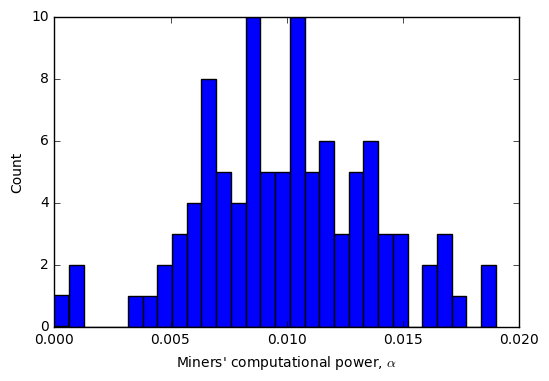
\includegraphics[width = .6\textwidth, height = 4cm]{figures/comp_pow.png}
\caption{Distribution of simulated miners' computational power in Simulation I.}
\label{fig:com_pow}
\end{figure}

We generated $N_{rounds} = 25$ simulations rounds for a number of selected parameters
for the levels of premium for loyalty, $\beta \in \{0.1, 0.5, 1.0,  2.0, 5.0, 10.0\}$, 
and for the miner's beliefs on the stability of the pool, 
$\gamma \in \{0.5, 0.6, 0.8, 0.9, 0.95, 0.99\}$. The goal of this set of simulations
is to test whether the badge system provides enough of incentives for the miners to stay
inside the pool rather than to jump to a proportional pool, when the round takes longer
than usual. We also are able to compute the average per share revenue of a loyal miner 
who stays in the pool throughout the whole extent of the round.

Fig.\ref{fig:pool_size} (a) and (b) show the pool size in terms of the number of
retained miners as the round gets longer. As expected the loyalty system
does not completely guard against miners' exiting to other pools with proportional
rewards system that have just opened a new round. However, as we see in 
Fig.\ref{fig:pool_size} (a) the higher the loyalty premium, $\beta$, the longer the miners stay in the badge pool, with $\beta = 5.0$ or $10.0$ resulting in almost
all miners remaining in the pool until the actual closing of the round.
The size of the pool over time also depends on the miners' beliefs on the pool's
stability. That is, the more the miner believes that the others are likely to leave 
the badge pool, the more he would be willing to stay in the pool, as he thinks
fewer shares will belong to people holding a badge. If at the end of the round
everyone has a badge, there would be no advantage from owning it. However, it
is still worth joining a badge pool at the beginning, as there is always
a probability that some miner would leave the pool before the round closing,
as people might exit even due to irrational reasons.


\begin{figure}[H]
\center
\subfloat[][Varying loyalty premium, $\beta$]
{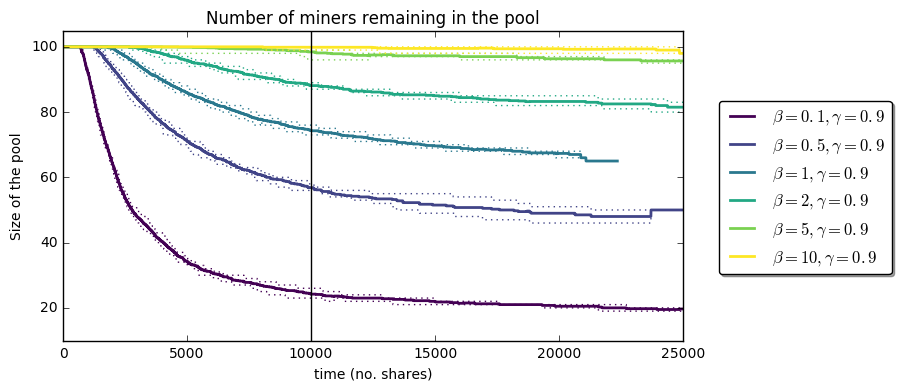
\includegraphics[width = .8\textwidth]{figures/pool_size_beta.png}}\\
\subfloat[][Varying belief on average miner's loyalty, $\gamma$]
{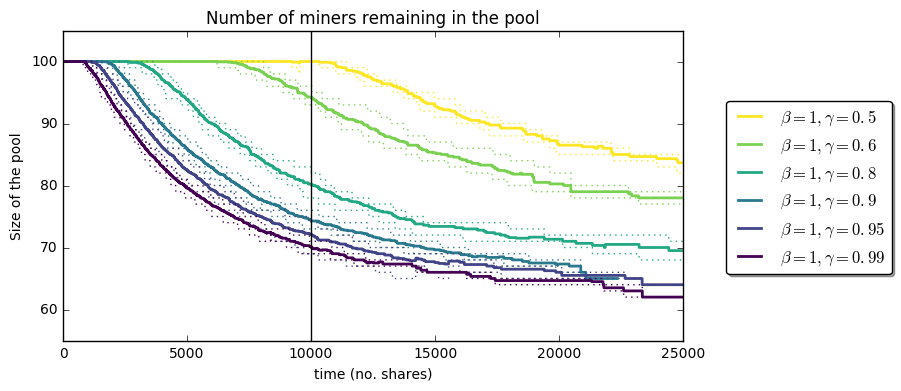
\includegraphics[width = .8\textwidth]{figures/pool_size_gamma.png}}
\caption{Number of miners remaining in the pool (out of 100)
with increasing number of shares submitted with a round.
Each solid line a mean, and dotted lines are min and max over 25 simulation 
runs. The $\beta$ parameter corresponds to the level of bonus assigned to 
loyal miners, and $\gamma$ to the belief of miners on the fraction 
of the number of current miners that will stay in the pool until the end
of the round. Vertical line marks the expected length of a round equal to 
difficulty, $D$.}
\label{fig:pool_size}
\end{figure}

We also look at the loyal miners' actual realized
revenue per share obtained at the end of the round. 
The revenues per share averaged over all loyal miners
across different $\beta$ levels are depicted in Fig.\ref{fig:loyal_rev}.
Consistent with the intuition, the higher revenues per share
are obtained from shorter rounds. We see that the revenue
can drop below the payout in a proportional pool with
an expected round length, $D$, if the round takes 
unusually long. However, the loss is not large, as
the loyal miners are compensated by the ones who
decided to exit the pool. We also observe that 
the premium level, $\beta$ should be set to be at least $1$
in order for the system to be effective and stable.
Note that with $\beta = 0.1, 0.5$ we have high volatility.
Moreover, with $\beta = 0.1$, the revenue for the loyal miners 
seems less predictable and does not closely correlate
to the length of a round (as should be expected).

\begin{figure}[h]
\center
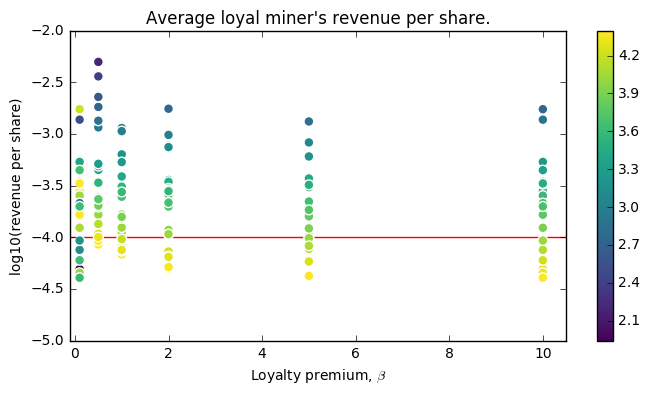
\includegraphics[width = .7\textwidth]
{figures/loyal_miners_revenue.png}
\caption{Average loyal miner's revenue per share ($\log_{10}$ scale)
in each round dependent on the premium level, $\beta$. Here we set 
$\gamma$ fixed at $0.9$. 
The colors correspond to the actual length of the round measured
as $\log_{10}$ of the total number of shares submitted. The red line
denotes the expected per share revenue from a proportional pool, equal
to $1/D$ as on average a round has $D$ submitted.}
\label{fig:loyal_rev}
\end{figure}

Overall, we observe promising patterns, that match the 
desired miners' behavior. Since our reward system directly punishes 
miners for leaving the pool, as anticipated fewer miners decide
to leave the pool in the middle of a long round. In the next step
we will simulate an entire Bitcoin ecosystem, whereas in the simulations
so far discussed we only allowed miners to make decisions which involve
comparing their expected revenue by staying in the pool versus
that o leaving to a proportional pool with a newly opened round.
This is of course idealistic, since there might not be any
pools with a new or so far short round available. Thus, a miner
might not even be able to jump to another pool. In the next
section we discuss another set of simulations that model 
an ecosystem with multiple pools present.


\subsection{Simulation II: the Bitcoin ecosystem}
In these simulations we specify the total number of miners $N_m$ as well as the total number of pools $N_p$. To determine each miner's computational power, we draw i.i.d. uniform random variables and then normalize. Initially, we place each miner into a pool uniformly at random. We also specify a hop percentage $h$, which is the fraction of the population that potentially engages in pool-hopping behavior. This group, chosen as simply the first $h$ fraction of miners, may hop between pools during the simulation, while everyone else must remain fixed during the entire simulation.

At each step of the simulation, a single miner wins a single share, with probability proportional to his own computational power. The share is then counted towards the round for the pool in which the miner is currently located. With probability $1/D$, that share is a block and the round for that pool ends and a reward is distributed. The parameter $D$ is chosen and fixed at the beginning of the simulation. After each step, the hopping population may hop between pools if they believe another pool is more enticing. The length of the simulation is $T_1+T_2$ steps, both parameters are specified at the beginning. In the first $T_1$ steps, no hopping is allowed by anyone. This short phase is just used to set up a random initial state of the system. If $T_1 = 0$, the initial state of the system is all pools beginning new rounds. If $T_1 > 0$, each pool will probably be in different length rounds, so we use this value to simulate a more realistic initial state of the system. Then in the second phase, consisting of $T_2$ steps, we allow hopping.

We focus on simulations for three different types of pools: a loyalty pool with a simple badge system, a PPLNS pool and a simple proportional pool. For the badge pools, the parameter $\beta$ is chosen at the beginning and fixed for the simulation, while for PPLNS pools, $N$ is treated in the same way. For all simulations discussed, we use $N=D$. 

The hopping miners must make a decision about which pool to join (or to remain in the same pool) at each step of the simulation. We model this decision by comparing expected revenues the miner would earn in each pool over the next $D$ shares found in that pool. On expectation, one block is found in this time frame. The expected revenue ($R$) for a miner with computational power $\alpha_i$ in a proportional pool $P_j$ with $S$ shares already found in a round is approximately given by:
\begin{equation*}
\mathbb{E}[R] \approx \left(\frac{\alpha_i}{\mathbb{E}[\sum_{k \in P_j}\alpha_k]} \right) \frac{C}{S+D}
\end{equation*}
where $\mathbb{E}[\sum_{k \in P_j}\alpha_k]$ is the expected computing power of the pool during the round. The miner does not necessarily know this value when making his decision, so in our simulations we assume the miner approximates this value with the computational power of the pool without any hoppers, that is, the computational power of the people who are always in that pool. This approximation will closely resemble but slightly underestimate the true value.

Similarly, the expected revenue for a miner with computational power $\alpha_i$ in a PPLNS pool $P_j$ with $S$ shares already found in a round is approximately given by:
\begin{equation*}
\mathbb{E}[R] \approx \left(\frac{\alpha_i}{\mathbb{E}[\sum_{k \in P_j}\alpha_k]} \right) \frac{C}{N}
\end{equation*}
where we make the same approximation on expected computing power as above. Finally, the same quantity for the badge pool is given by:
\begin{equation*}
\mathbb{E}[R] \approx \left(\frac{\alpha_i}{\mathbb{E}[\sum_{k \in P_j}\alpha_k]} \right) \cdot \left(\frac{C(1+\beta \mathbbm{1}_B)}{(S+D)(1+\beta \frac{S_B}{S})} \right)
\end{equation*}
where $\mathbbm{1}_B$ is the indicator variable that miner $i$ qualifies for a badge currently and $S_B$ is the number of shares owned by miners qualifying for a badge currently. Note that we are setting the $\gamma$ parameter from our earlier discussion to 1 in this decision. The miner assumes all potential badge qualifiers, except possibly himself, remain in the pool. We may do this because here we are dealing with unequal pool sizes, unlike in our previous analysis. If a miner is currently qualified for a badge and already has $x$ shares, then the expected revenue he forfeits by hopping from the badge pool is:
\begin{equation*}
\mathbb{E}[R_f] = C x \cdot \left(\frac{1+\beta}{(S+D)(1+\beta \frac{S_B}{S})} -\frac{1}{(S+D)(1+\beta \frac{S_B-x}{S})}\right)
\end{equation*}
Thus at each step, we compute these expected values for each prospective pool (the expected forfeited revenue only if the miner is currently in a badge pool and qualifies for a badge) and let the miner hop to the pool with the maximum expected revenue. For example, a miner in the badge pool currently who is qualified for a badge will only hop to another pool if the expected revenue of that pool exceeds the expected revenue of the badge pool by more than the revenue forfeited for hopping.

\begin{figure}[H]
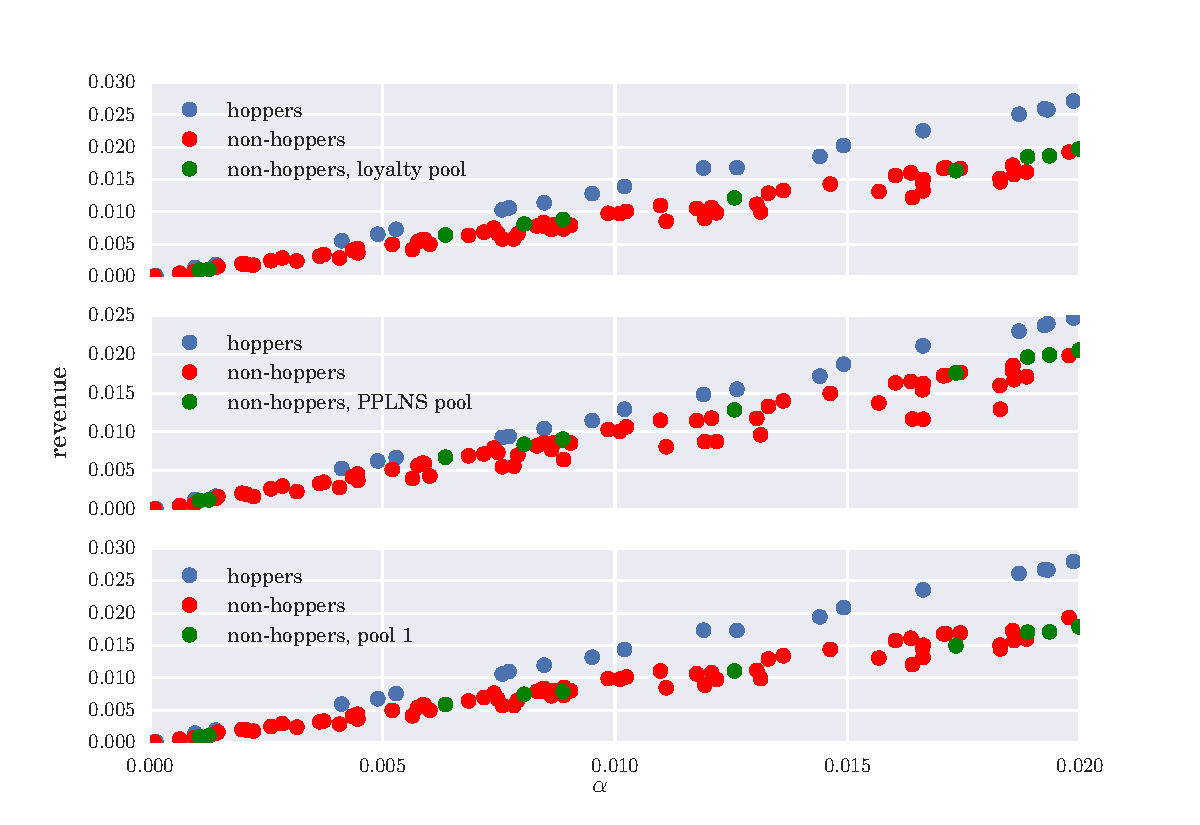
\includegraphics[width = \textwidth]{figures/compare_revs2.pdf}
\caption{Example simulation with 7 pools, 100 miners, $h = 0.2$, $D = 250$, $T_1 = 500$ and $T_2 = 2000T_1$. Each simulation had the same distribution of miners and pools as well as share winners. The type of reward system of pool one differs in each plot - badge system with $\beta = 1$ (top), PPLNS system with $N=D$ (middle) and proportional system (bottom) - while the other six pools are proportional reward pools.}
\label{fig:compare_revs}
\end{figure}

Fig.~\ref{fig:compare_revs} shows a single simulation for three different ecosystems. In each of these three systems, we have seven pools. We fix the last six to be proportional scheme pools while we vary the type of the first pool. One system has a badge system with $\beta = 1$, one has a PPLNS system with $N=D$ and the other is just another proportional system. The plots show the amount of revenue earned by each miner compared to his computational power during the simulation. Without hopping, these values should be equivalent. However, we see that with hopping, the miners who hop are able to earn more than their share of revenue in all three systems. These results show that pool-hopping can still be beneficial in systems with at least one PPLNS pool. In this simulation, the PPLNS is harsher on hoppers than our badge pool is, giving less advantage, but both do better than the all proportional system, as we expect. Furthermore, we see that in both the PPLNS and badge pools, the miners who are fixed to that particular pool fare better than they do than if they were in a proportional pool, which helps solve one of our main motivations for preventing pool-hopping. 

\begin{figure}
\subfloat[]{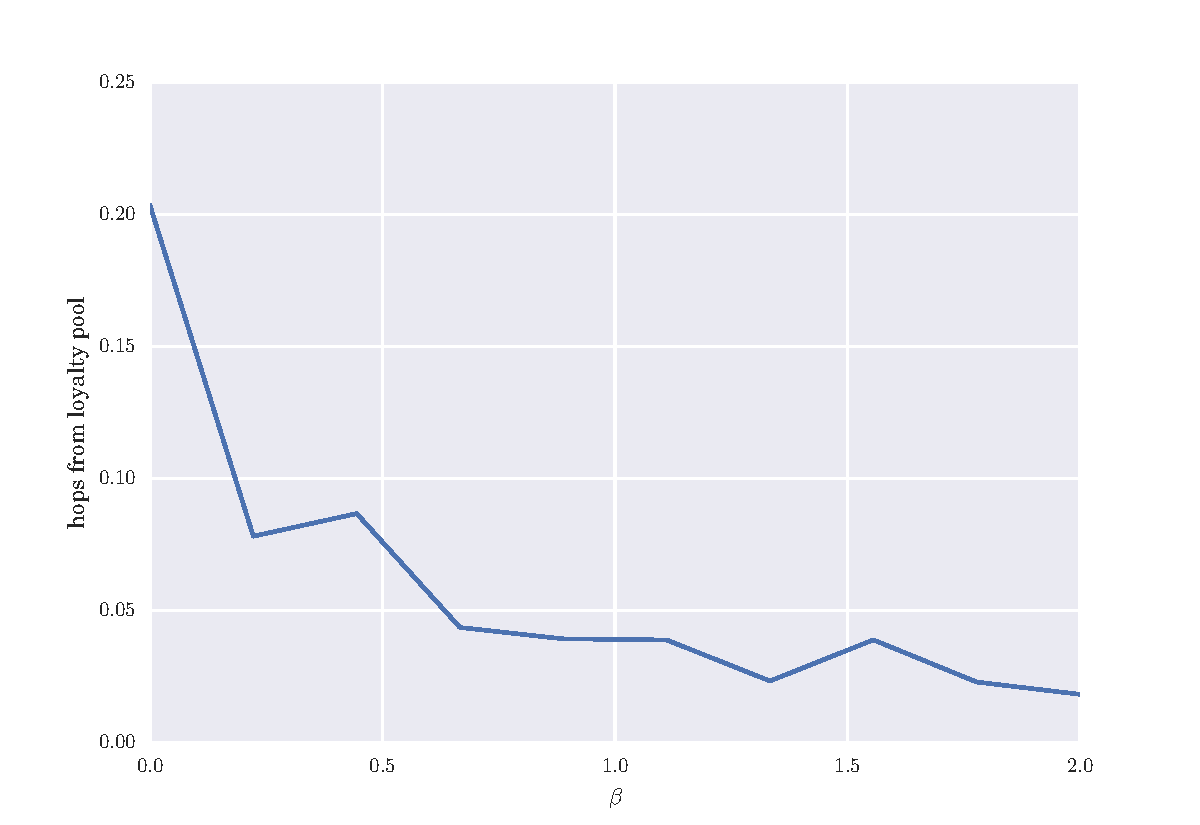
\includegraphics[width = .5\textwidth]{figures/hop_frac.pdf}}
\subfloat[]{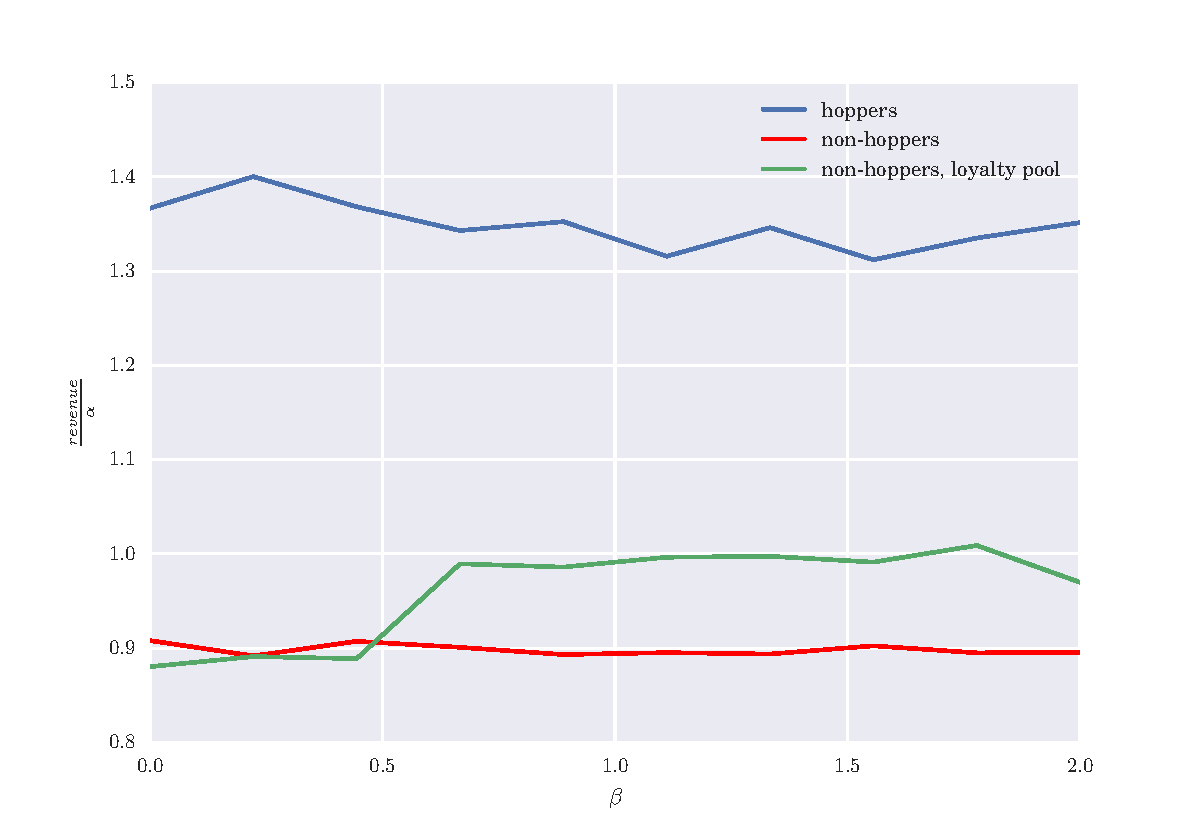
\includegraphics[width = .5\textwidth]{figures/badge_revs.pdf}}
\caption{Simulations with one badge pool and 4 proportional pools with varying $\beta$. Parameters are: $N_m = 100$, $D = 200$, $h = 0.2$, $T_1 = 1000$ and $T_2 = 100T_1$ with 25 simulations per $\beta$. On the left, we see the fraction of hops involving people leaving the badge pool. On the right we see the ratio of revenue to computational power for each type of miner.}
\label{fig:vary_beta}
\end{figure}

We examine the effect of the badge bonus parameter $\beta$ in Fig.~\ref{fig:vary_beta}. We create a system with five pools, all proportional except a single badge pool with parameter $\beta$, and run 25 simulations for various values of $\beta$. Notice that the average fraction of hops leaving the badge pool decreases with increasing $\beta$ (Fig.~\ref{fig:vary_beta}a). This result matches our expectation; as $\beta$ increases, the cost of leaving the badge pool in the middle of a round increases if a miner already has shares in the round. We always expect miners with no current shares during a long round to leave the badge pool for a proportional pool with a newer round, but with large $\beta$ we can prevent people from making this jump even if the they only have a few shares in the round currently.

For these simulations, we also track the average ratio of revenue to computational power for every miner. We see that as $\beta$ increases, some revenue shifts from the hoppers to the non-hoppers in the badge pool, as the higher punishment for leaving the badge pool rewards those who remain. This revenue re-distribution lessens with increasing $\beta$ as well, because the number of people hopping from the badge pool decreases. The revenue ratio of non-hoppers in the badge pool approaches 1, an outcome we desire, while the other non-hoppers revenue ratio stays constant around 0.9 for all $\beta$. So our badge pool insulates the non-hoppers from being harmed by the hoppers. 

We also run 25 simulations on the same system, changing the badge pool (pool 1) to a PPLNS pool and then to a proportional pool. The following table shows the revenue rates for each miner type as well as the fraction of hops leaving pool 1 for each new system.

\begin{table}
\begin{center}
\begin{tabular}{ |c|c|c|c|c| } 
 \hline
 & hoppers & non-hoppers (pool 1) & non-hoppers (other) & hop-from fraction \\ 
 \hline
 Badge ($\beta = 5$) & 1.351 & 1.004 & 0.891 & 0.018 \\
 \hline
 PPLNS & 1.226 & 0.976 & 0.918 & 0.045 \\ 
 \hline
 Proportional & 1.414 & 0.871 & 0.898 & 0.379\\ 
 \hline
\end{tabular}
\end{center}
\caption{Simulations with one pool as specified on the left and 4 proportional pools. Parameters are: $N_m = 100$, $D = 200$, $h = 0.2$, $T_1 = 1000$ and $T_2 = 100T_1$ with 25 simulations per system. Shows average ratio of revenue and computing power for each type of miner as well as the fraction of hops during the simulation that involve leaving pool 1.}
\end{table}
Again, we see that hoppers benefit in both environments still. These results give more evidence that pool-hopping may still be beneficial in Bitcoin ecosystems that involve both PPLNS and proportional pools. Like our badge system, the PPLNS system redistributes revenue from the hoppers to the non-hoppers in the PPLNS pool, but the two systems achieve this outcome in very different manners. For modest values of $\beta$, our badge system does just as well as PPLNS at preventing hopping from the pool. The badge system achieves very similar results as the PPLNS system, though it performs slightly worse at dampening the revenue rate of pool-hoppers. Overall, we see with these simulations, in order to prevent all or most pool-hopping, most pools must adopt some sort of anti-hopping system; a large number of proportional pools will always encourage hopping behavior. 

\section{Conclusion and Future Work}
Bitcoin miners tend to form mining pools in order to decrease the variance of their revenue streams. Pools are governed by reward functions to distribute rewards to their miners for each found block. Reward functions in which payoffs depend only on the length of the round, such as proportional schemes, are especially vulnerable to pool-hopping strategies, as we show in simulations. Pool-hopping, while beneficial to the hopper, may harm both the non-hopping population as well as the pool managers. Some pools utilize PPLNS and other score-base methods to prevent hopping by standardizing the round length, and thus getting rid of payoff structures that depend on round length. Through simulations, we show that while PPLNS does combat some of the advantages of pool-hopping and minimize some of the collateral harm done, miners who switch pools may still benefit financially. 

In this paper we develop a new class of reward functions based on loyalty to discourage pool-hopping. These methods explicitly penalize miners who leave a pool mid-round by devaluing their shares already contributed. We give analysis and simulations for one such method, the badge based system, as well as discuss other functions in the class. Simulations show that this system does help prevent hopping and importantly protects miners in the pool who choose not to hop from losing revenue to the hoppers. It performs similarly, though slightly less effectively, to PPLNS at hop prevention. However, we achieve this very similar behavior through a fundamentally new technique; instead of standardizing the round length to eliminate payoff dependencies on it, the badge system leaves payoff dependencies on round length but also adds a payoff dependency on loyalty. Furthermore, these ideas may be combined with scoring based methods very easily. For this reason, we believe this new class of reward functions is very promising. 

Hybrid methods that combine scoring with loyalty should help prevent hopping very well. In the future, we would like to analyze these functions. Additionally, this work focuses on simulations with a single hop-prevention pool; ecosystems with multiple hop-prevention pools should see less advantages for pool-hopping, so a more robust treatment of these methods with simulations would be enlightening. Finally, we only discuss reward functions for single rounds. We may easily extend this concept of loyalty to span multiple rounds. In this case for example, pool managers can give out a badge bonus to a miner who has stayed in the pool for a specified number of rounds. We have done some work on this problem and believe it would yield some interesting results.

\bibliographystyle{plain}
\bibliography{project}
\end{document}